% tex file for convolution
\par \indent Our study is structured around event-related neurological 
stimulus, not block stimulus as was discussed as the in-class example. We 
predicted the hemoglobin response (HR) related to this type of neurological 
stimulus, since the methods in class were much better for block stimulus. 
Moreover, our stimulus (as is the case in event-related stimulus studies) was 
not evenly split. We developed a few other functions to take this into 
account, and will likely implement additional procedures in the future.

\par The three approaches that we are in the process of exploring address 
modeling the HR from the neural stimulus. The first two have already been 
completed. \textbf{(1)} We first implemented the standard block-stimulus 
paradigm related \texttt{np.convolve} function (which failed to take into 
account the non-trivial times of stimulus). \texttt{np.convolve} utilities 
FFT (Fast Fourier Transforms). \textbf{(2)} Next, we developed a function 
that does not utilize FFT, but allows for discontinuous stimulus events 
(discontinuous being non-uniform stimulus timing in this scenario). We used a 
continuous HR function to model the response (whereas \texttt{np.convolve} 
uses a discrete HR function).\textbf{(3)} Our next project will be to utilize 
the strength of FFTs by splitting up the time into 60 milliseconds intervals 
(a very small time metric), and then uses \texttt{np.convolve} and some 
rounding of the stimulus response occurrences to get another candidate for 
the hemoglobin response related to the neurological stimulus. This procedure 
would take advantage of FFTs, and would not be hindered by assumptions of 
time, since the HR model is not extremely precise and has a good amount of 
variance.
    
\par For \textbf{(2)} and \textbf{(3)} we had to scale back down to the image 
capturing time frame (2 seconds) [Figure \ref{fig:convolution}].

\begin{figure}[ht]
\centering
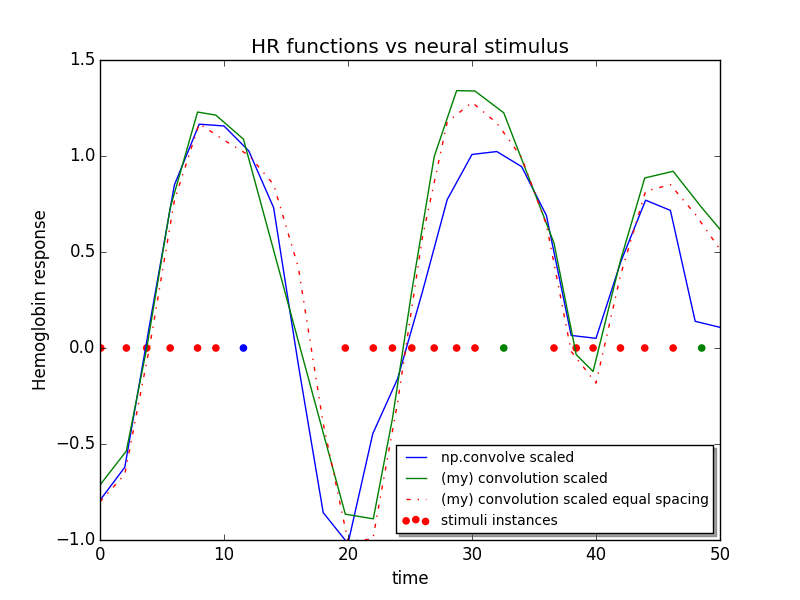
\includegraphics[scale=0.5]{images/convolution_vs_neural_stimulus} 
\caption{Different convolution function vs the Nueral stimulus}
\label{fig:convolution}
\end{figure}

